Essa seção tem como objetivo delimitar o escopo deste trabalho, apresentar os fundamentos teóricos pertinentes e apresentar a aplicação que será construída como estudo de caso:

\section{Proposta}

Contratos inteligentes que são hospedados em uma rede baseada na tecnologia blockchain precisam ser alimentados com dados para executarem suas ações pré-programadas. Devido as limitações dos dispositivos modernos em enviar seus dados diretamente para redes do tipo blockchain, bem como o alto custo para manter tais dados na rede blockchain, faz-se necessário a utilização de microserviços que intermediem o envio de dados e que também armazenem parte dos dados utilizados pelos contratos, reduzindo-se o custo de armazenamento no blockchain.

O Objetivo deste trabalho é comparar a nível de performance, custo, confiabilidade, segurança e privacidade os prós e contras de duas arquiteturas para uma mesma aplicação baseada em um contrato inteligente:

\begin{itemize}
\item Arquitetura 1 (figura \ref{arquitetura_1_generica}): Nessa arquitetura, todos os dados necessários para a execução do contrato inteligente estão no blockchain.
\item Arquitetura 2 (figura \ref{arquitetura_2_generica}): Nessa arquitetura parte dos dados necessários para a execução do contrato inteligente se encontra no blockchain e outra parte dos dados se encontra em um banco de dados tradicional administrado pela pessoa ou instituição responsável pela aplicação.
\end{itemize}

\begin{figure}[ht]
\centering
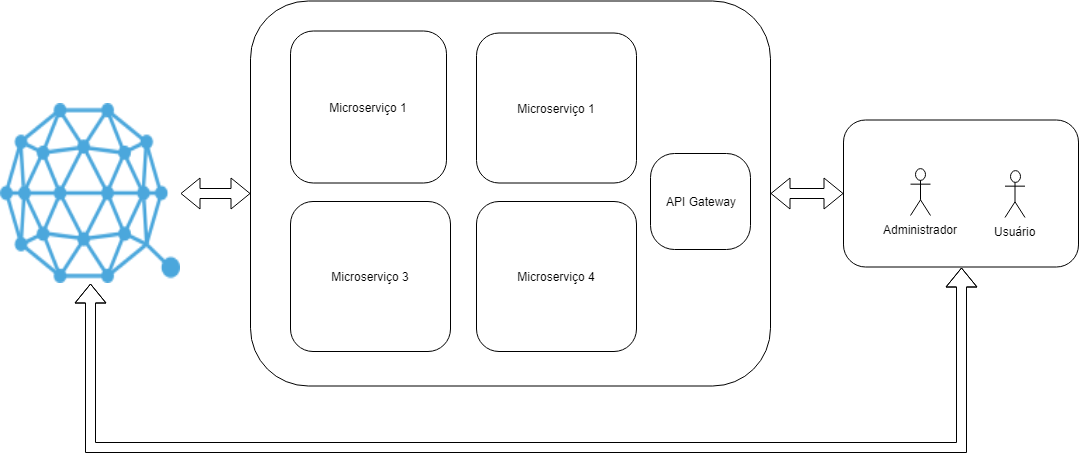
\includegraphics[width=0.7\textwidth]{Cap1/arquitetura_1_generica}
\caption{Arquitetura 1: Todos os dados pertinentes ao contrato estão no blockchain.}
\label{arquitetura_1_generica}
\end{figure}

\begin{figure}[ht]
\centering
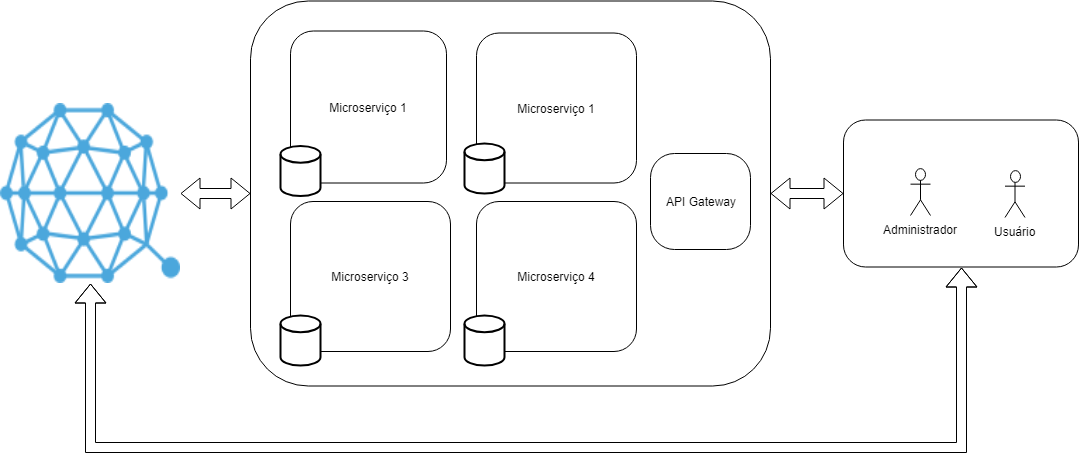
\includegraphics[width=0.7\textwidth]{Cap1/arquitetura_2_generica}
\caption{Parte dos dados está no blockchain e outra parte dos dados está em um banco de dados tradicional.}
\label{arquitetura_2_generica}
\end{figure}

Devido ao grande número de redes blockchain que suportam contratos inteligentes, bem como o grande número de aplicações que podem ser construídas com o uso de contratos inteligentes, a comparação das duas arquiteturas propostas será feita especificamente para uma aplicação de um seguro automotivo baseado em um contrato inteligente hospedado no blockchain Ethereum.

\section{Blockchain 1.0}

Blockchain 1.0 se refere a aplicação do blockchain para construção de moedas digitais, cryptomoedas \cite{blockchainneweconomy}. A mais famosa delas é o Bitcoin, cuja especificação técnica se encontra no paper de Satoshi Nakamoto \cite{paper_satoshi}. Nesta seção será explicado os mecanismos básicos do blockchain 1.0 especicíficos do Bitcoin.

\subsection{O Paper de Satoshi Nakamoto}

Neste paper, Satoshi Nakamoto propõem a construção de uma moeda digital, Bitcoin, baseada em uma rede peer to peer, na qual as transações são assinadas digitalmente e o problema do gasto duplo é resolvido por meio da construção de uma cadeia de blocos que armazenam as transações em ordem cronológica. A construção e aceitação de tais blocos é feito de modo que se mais da metade do poder de processamento da rede em questão for honesto, as transações serão válidas.

\subsection{Transações}

De uma forma simplificada, cada transação de certa quantia de bitcoin no blockchain 1.0 conterá \cite{bitcoin_transaction}:

\begin{itemize}
\item O hash da transação anterior, que transferiu o bitcoin para o dono atual
\item A chave pública do dono atual do bitcoin
\item A assinatura do dono atual do bitcoin sobre o hash de uma versão simplificada da transação
\item O hash da chave pública do futuro dono do bitcoin
\item A quantia de bitcoin que será transferida na transação em questão
\end{itemize}

\begin{figure}[ht]
\centering
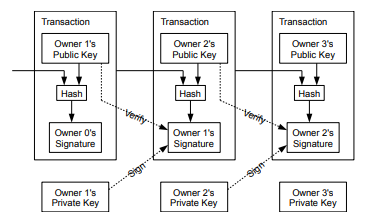
\includegraphics[width=0.5\textwidth]{Cap1/blockchain_transactions}
\caption{Transações em um blockchain.}
\label{blockchain_transactions}
\end{figure}

Apesar dessa solução garantir que uma transação ocorra apenas se o dono dela autorizar, por meio de uma assinatura ECDSA (Elliptic Curve Digital Signature Algorithm). Ela ainda não resolve o problema do gasto duplo. Para resolver esse problema, todos os nós da rede devem estar cientes de todas as transações e em caso de gastos duplo, os nós também concordar qual será considerada a transação válida.

\subsection{Servidor Timestamp}

Para evitar o problema do gasto duplo, o bitcoin utilizar um servidor timestamp, que faz com que as transações sejam agrupadas em blocos e cada bloco possuirá seu hash, que dependerá do hash do bloco anterior, das transações dentro daquela bloco e do tempo no qual aquele bloco foi criado. Dessa forma, cada nó garante uma ordem cronológica na ocorrência das transações e pode, em caso de gasto duplo, determinar qual transação será considerada a transação válida.

\begin{figure}[ht]
\centering
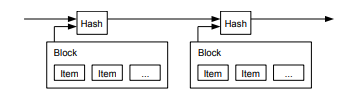
\includegraphics[width=0.5\textwidth]{Cap1/blockchain_timestamp}
\caption{Servidor Timestamp.}
\label{blockchain_timestamp}
\end{figure}

\subsection{Prova de Trabalho}

Para garantir concordância entre os nós da rede, a cadeia de blocos mais longa é considerada como sendo a verdadeira. Para evitar que algum nó crie uma transação inválida ou modifique uma transação anterior, a criação de cada bloco exige que o nó que está criando aquele bloco varie certos valores do bloco de modo que o hash do bloco inicie com determinado número de zeros. Como o hash de cada bloco depende do hash anterior, se algum nó quiser adicionar uma transação inválida ou modificar um bloco anterior, ele deverá construir os blocos mais rápidos que os outros nós da rede. 

Dessa forma, cada nó da rede que participa da criação de blocos (mineradores) fica variando certos valores do bloco até encontrar um hash válido ou até um outro nó encontre um hash válido antes dele.

\begin{figure}[ht]
\centering
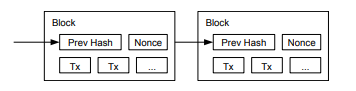
\includegraphics[width=0.5\textwidth]{Cap1/pow}
\caption{Prova de trabalho.}
\label{pow}
\end{figure}

O número de zeros que o hash de cada bloco deve ter é ajustado de modo que a criação de cada bloco leve em média 10 minutos, conforme pode-se observar na figura \ref{block_avg_time} \cite{time_avg_block}.

\begin{figure}[ht]
\centering
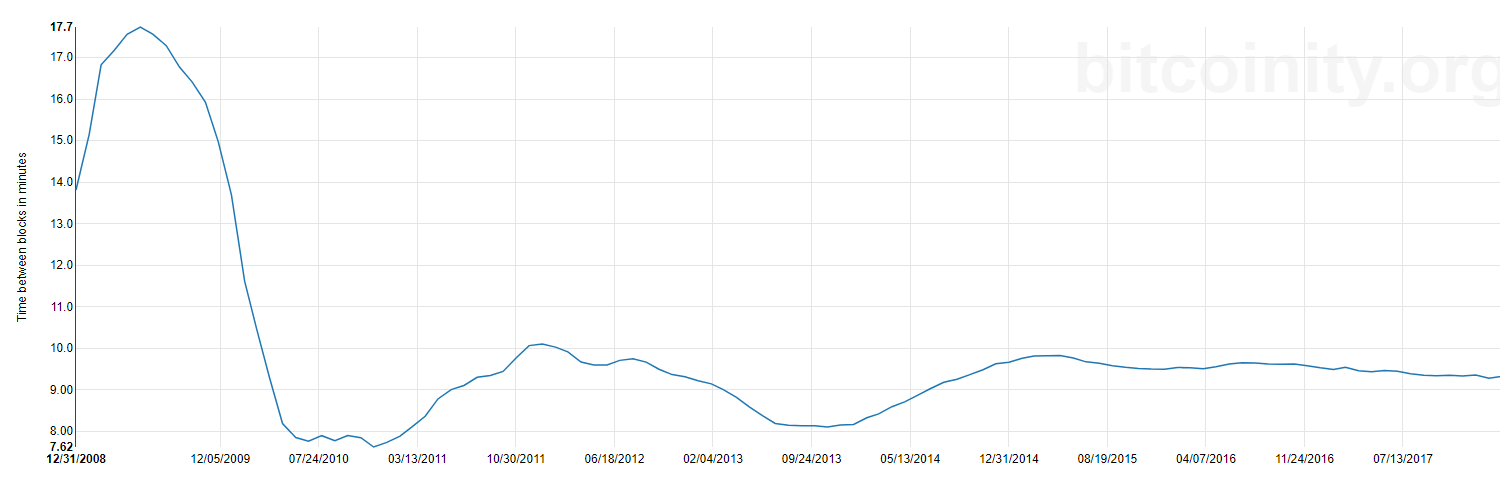
\includegraphics[width=1\textwidth]{Cap1/block_avg_time}
\caption{Tempo de geração de um novo bloco.}
\label{block_avg_time}
\end{figure}

\subsection{Rede}

Os nós de uma rede blockchain 1.0 apresentam o seguinte comportamento \cite{paper_satoshi}:

\begin{itemize}
\item Novas transações são emitidas para todos os nós
\item Cada nó coleta as transações em um bloco
\item Cada nó trabalha para encontrar o hash do seu bloco, prova de trabalho
\item Quando um nó encontra sua prova de trabalho, ele emite o bloco para todos os nós
\item Cada nó aceita um bloco apenas se todas as transações forem válidas (assinadas e sem gastos duplos)
\item Ao aceitar um bloco, os nós começam a trabalhar na prova de trabalho do próximo bloco, considerando o hash do último bloco aceito.

\end{itemize}

\subsection{Incentivo}

Para incentivar a entrada e permanência de novos nós na rede e introduzir novas moedas bitcoins ao mercado, cada novo bloco criado gerará uma certa quantia de bitcoins que poderá ser creditada em uma conta determinada pelo nó que resolveu a prova de trabalho do bloco em questão.

\subsection{Combinando e Particionando Valor}

A origem dos bitcoins em cada transação pode advir de múltiplas saídas de outras transações, bem como cada transação pode conter múltiplos destinos para o envio dos bitcoins.

\begin{figure}[ht]
\centering
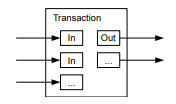
\includegraphics[width=0.3\textwidth]{Cap1/value_partition}
\caption{Combinando e particionando valor.}
\label{value_partition}
\end{figure}

\subsection{Privacidade}

Como o credor e creditado de cada transação é específicado por uma chave pública, não há como determinar a identidade das pessoas/instituições que fazem/recebem as transações. Desse modo, em uma rede blockchain 1.0, as transações são públicas, mas a identidade das pessoas/instituições é preservada.

\section{Blockchain 2.0}

Blockchain 2.0 se refere a aplicação do blockchain para construção de contratos inteligentes \cite{blockchainneweconomy}. A blockchain 2.0 mais famosa é a Ethereum, cuja proposta se encontra no paper escrito por Vitalik Buterin \cite{paper_ethereum}.

\subsection{O Paper de Vitalik Buterin}

Neste paper, Vitalik propõem a criação de uma nova versão do blockchain. Ele mostra que o blockchain pode ser visto como uma máquina de transição de estados e extende o conceito de blockchain de Nakamoto criando o Ethereum, uma rede blockchain na qual cada mudança de estado é executada por uma máquina virtual Turing-completa. Em uma rede blockchain 2.0 como Ethereum, além de armazenar dados de transações monetárias (na moeda Ether) ela também é capaz de armazenar e de processar qualquer tipo de dado, aumentando assim a gama de aplicações possíveis.

\begin{figure}[ht]
\centering
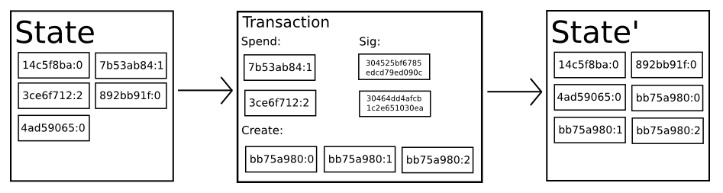
\includegraphics[width=0.8\textwidth]{Cap1/blockchain_as_state_transition_machine}
\caption{Blockchain como uma máquina de transição de estados.}
\label{blockchain_as_state_transition_machine}
\end{figure}

\subsection{Aplicações com Ethereum}

A possibilidade de se executar código no blockchain possibilita a criação de diversas aplicações, entre elas:

\subsubsection{Sistemas de Token}

Sistemas de token são como moedas de troca para um determinado ecossistema e possuem como operação básica a transferência do token de uma conta para outra:

\begin{minted}{python}
def send(to, value):
    if self.storage[msg.sender] >= value:
        self.storage[msg.sender] = self.storage[msg.sender] - value
        self.storage[to] = self.storage[to] + value
\end{minted}

\subsubsection{Domain Name Service}

Uma outra aplicação para o Ethereum é construção de uma base de dados pública para o armazenamento de domínios, o contrato dessa aplicação possuiria uma operação para registrar novos domínios:

\begin{minted}{python}
def register(name, value):
    if not self.storage[name]:
        self.storage[name] = value
\end{minted}

\subsection{Contas no Ethereum}

No Ethereum, toda transição de estado é marcada pela transição de valor ou dado de uma conta Ethereum. Toda conta Ethereum possui quatro campos:

\begin{itemize}
\item Nonce: Inteiro incrementado em cada transação da conta em questão
\item Balanço: A quantia de Ether que essa conta possui
\item Contrato: Código de contrato dessa conta, caso possua
\item Storage: Contém os dados persistentes dessa conta
\end{itemize}

Conforme pode-se observar nos campos acima, uma conta Ethereum pode ser gerenciada por uma pessoa ou por um código. No caso em que a conta é gerenciada por um código, diz-se que a conta é um contrato.

\subsection{Mensagens e Transações no Ethereum}

Transações podem enviar Ether para uma conta ou então ativar o contrato de alguma conta. Toda transação deve ser assinada por seu emissor e possui os seguintes campos:

\begin{itemize}
\item O receptor da transação
\item A assinatura identificando o emissor
\item A quantia de Ether que será fornecida
\item Startgas: Valor que representa quantos passos computacionais essa transação está permitida a fazer
\item Gasprice: Valor que representa o quanto o emissor está disposto a pagar por passo computacional
\end{itemize}

Para evitar loopings infinitos sendo executados nos contratos, cada transação deve fornecer uma quantia de Ether proporcional à quantia de passos computacionais que tal transação consumirá. Dessa forma, se algum usuário malicioso criar um contrato com um looping infinito e atrasar o processamento da rede, ele terá que pagar por isso.

As mensagens são semelhantes às transações, porém são utilizadas para que contratos interajam com outros contratos.

\subsection{Função de Transição de Estado no Ethereum}

Uma transição de estado no Ethereum segue os seguintes passos:

\begin{enumerate}
\item Checa-se se a transação é válida: possui o número correto de parâmetros, a assinatura é válida e o nonce da transação corresponde ao nonce da conta.
\item Calcula-se a taxa da transação (\(STARTGAS * GASPRICE\)) e a debita o valor da conta do remetente da transação, bem como incrementa o nonce do remetente
\item Inicializa-se \(GAS = STARTGAS\) e debita de \(GAS\) o valor correspondente ao custo do transporte de dados da transação em questão
\item Transfere-se o valor especificado na transação do remetente para o destinatário, caso a conta destinatária não exista, ela é criada.
\item Caso o remetente não tenha fundos suficientes ou a execução do código já consumiu toda quantia de gás fornecida, todas as alterações em contas afetadas devem ser revertidas e as taxas de gas devem ser creditadas na conta de quem minerou o bloco.
\item Caso a transação ocorra normalmente, a quantia de ether em forma de gas que não foi consumida é creditada na conta do remetente da transação.
\end{enumerate}

\begin{figure}[ht]
\centering
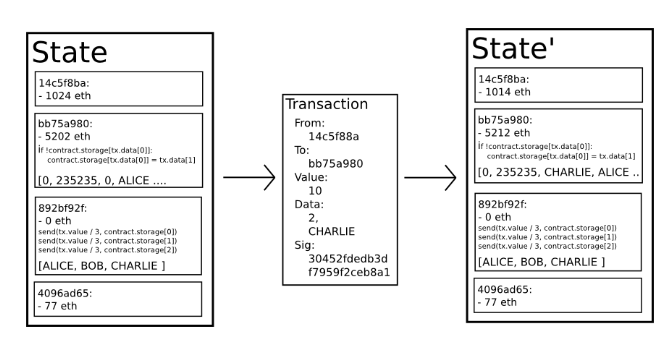
\includegraphics[width=0.8\textwidth]{Cap1/ethereum_state_transiction_function}
\caption{Diagrama de uma transição de estado no Ethereum.}
\label{ethereum_state_transiction_function}
\end{figure}

\subsection{Execução de Código no Ethereum}

Os códigos de contratos no Ethereum são criados em linguagens de alto nível, como Solidity (semelhante a JavaScript) e Serpent (semelhante a Python) e são compilados para uma linguagem de baixo nível em bytecode que será interpretada pela EVM (Ethereum Virtual Machine).

\begin{figure}[ht]
\centering
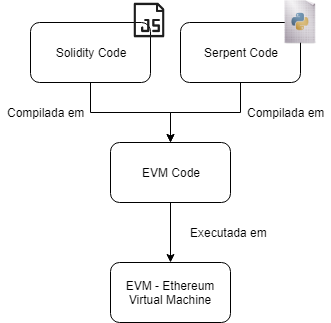
\includegraphics[width=0.5\textwidth]{Cap1/ethereum_compilation_and_execution}
\caption{Compilação e execução no ambiente Ethereum.}
\label{ethereum_compilation_and_execution}
\end{figure}

A EVM executa EVM code, uma linguagem bytecode de baixo nível baseada em pilha. O estado computacional da EVM é determinado a partir de 5 parâmetros \cite{ethereum_yellow_paper}:

\begin{itemize}
\item g: Quantia de gás disponível
\item pc: Contador do programa
\item m: Conteúdo na memória temporária
\item i: O número de palavras na memória
\item s: O conteúdo da pilha
\end{itemize}

\section{Microserviços}

De acordo com Sam Newman \cite{building_microservices}, uma arquitetura baseada em microserviços se dá por uma abordagem na qual uma aplicação é dívidida em n serviços com ciclo de vida próprio e com responsabilidades específicas. Tais serviços cooperam entre si e juntos formam a aplicação como um todo.

\subsection{Características desejáveis de um microserviço}

\begin{itemize}
\item Pequenos e focados em fazer apenas uma coisa: Os microserviços devem ser baseados em domínios de negócio da aplicação em questão, garantindo que a base de código de cada microserviço não cresça indeterminadamente e garantindo que os programadores saibam exatamente qual microserviço é responsável por determinada tarefa.
\item Autonomia: Cada microserviço pode ser colocado em produção de forma independente, os microserviços interagem entre si por meio de chamadas de API na rede.
\end{itemize}

\subsection{Vantagens de se utilizar microserviços}

\begin{itemize}
\item Heterogeneidade de tecnologia: Como cada microserviço é independente um do outro, cada microserviço pode ser constrúido com uma tecnologia específica. Por exemplo, o microserviço A pode utilizar a linguagem Python e um banco de dados relacional, como PostgreSQL. Já um segundo microserviço B, poderia utilizar a linguagem Go e um banco de dados não relacional, como MongoDB.
\item Resiliência: Se um microserviço falhar, a aplicação como um todo não será comprometida. Apenas o microserviço em questão e as funcionalidades que dependem dele estarão indisponíveis.
\item Facilidade para deploy: Ao alterar o código de um microserviço, pode-se colocar tal mudança em produção rapidamente com um risco menor de se inserir falhas, dado que você alterou apenas uma parte específica e isolada da aplicação.
\item Alinhamento Organizacional: A responsabilidade por cada microserviço pode ser atribuída a um time específico, tornando mais claro a responsabilidade de cada time e como os times devem se alinhar para interagirem com as funcionalidades criadas por outro time.
\item Otimizado para mudanças: Caso seja necessária uma mudança grande na aplicação, essa mudança será gradualmente implementada, um microserviço por vez, reduzindo os riscos de tal mudança.
\end{itemize}

\section{API's REST}

Devido à necessidade de escalabilidade, interação de componentes, generalidade de interface, independência de deploys e mudanças da World Wide Web, Roy Fielding formaliza \cite{royrest} a proposta de uma arquitetura que atenda tais necessidades. Tal arquitetura ficou conhecida como REST (REpresentational State Transfer) e é baseada em 6 pricípios:

\subsection{Modelo cliente-servidor}

Nesse modelo, cliente e servidor podem evoluir independentemente um do outro. As preocupações com a interface do usuário estarão desacopladas das preocupações com o armazenamento de dados, possibilitando interfaces de usuários em múltiplas plataformas com a mesma base de dados.

\begin{figure}[ht]
\centering
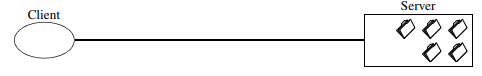
\includegraphics[width=0.5\textwidth]{Cap1/rest_client_server}
\caption{Modelo cliente-servidor}
\label{rest_client_server}
\end{figure}

\subsection{Stateless}

Cada request do cliente para o servidor deve conter toda informação necessária. Com isso aumenta-se a  visibilidade pois uma análise da interação cliente e servidor irá conter apenas um request. A confiabilidade do sistema também aumenta, pois o estado/sessão será mantido no cliente e qualquer problema no servidor não o afetará. Isso também aumenta a escalabilidade, pois o servidor não irá despender recursos para armazenar o estado/seção dos usuários.

\begin{figure}[ht]
\centering
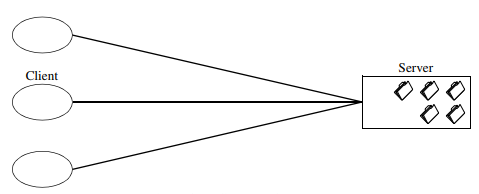
\includegraphics[width=0.5\textwidth]{Cap1/rest_stateless}
\caption{Stateless}
\label{rest_stateless}
\end{figure}

\subsection{Cache}

Para poupar os recursos de rede e/ou computação no servidor, quando o cliente ou servidor já possuir uma copia suficientemente atualizada do recurso requisitado, o recurso armazenado na cache será utilizado. Com isso aumentamos a escalabilidade do sistema e a percepção de velocidade pelo usuário final.

\begin{figure}[ht]
\centering
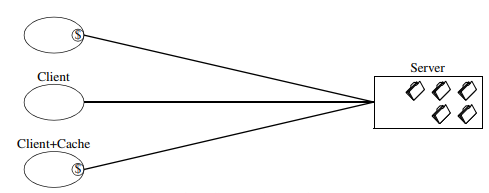
\includegraphics[width=0.4\textwidth]{Cap1/rest_cache}
\caption{Cache}
\label{rest_cache}
\end{figure}

\subsection{Interface Uniforme}

Ao definir e utilizar uma interface única para comunicação entre os componentes do sistema, a arquitetura do sistema é simplificada e compreende-lo se torna mais claro.

\begin{figure}[ht]
\centering
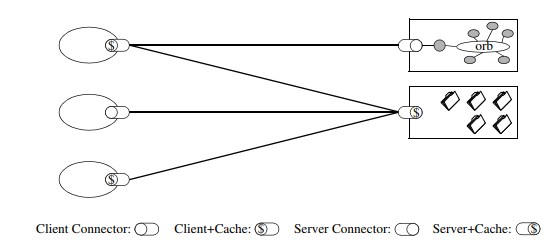
\includegraphics[width=0.5\textwidth]{Cap1/rest_uniform_interface}
\caption{Interface uniforme}
\label{rest_uniform_interface}
\end{figure}

\subsection{Sistema Baseado em Camadas}

Embora adicionem uma latência maior para o processamento de dados, um sistema baseado em camadas promove uma maior independência entre os componentes do sistema.

\begin{figure}[ht]
\centering
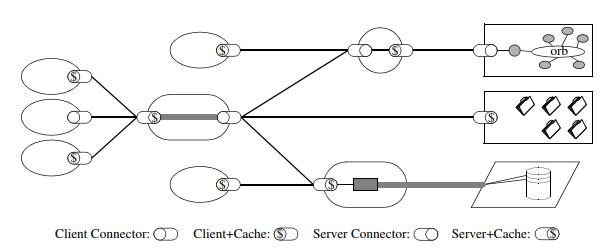
\includegraphics[width=0.5\textwidth]{Cap1/rest_layer_based_system}
\caption{Sistema baseado em camadas}
\label{rest_layer_based_system}
\end{figure}

\subsection{Código sob Demanda}

As funcionalidades e comportamentos dos clientes podem ser extendidos com o download de scripts que estão no servidor. Dessa forma, o cliente é simplificado, no sentido de exigir uma menor quantia de features pré-implementadas.

\begin{figure}[ht]
\centering
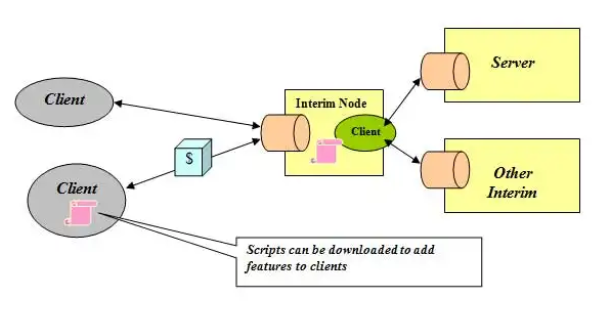
\includegraphics[width=0.5\textwidth]{Cap1/rest_code_on_demand}
\caption{Código sob demanda}
\label{rest_code_on_demand}
\end{figure}

\section{Estudo de Caso: Um seguro automotivo baseado em um contrato inteligente}

A aplicação que será construída e que proverá os dados para análise e comparação é a de um seguro automotivo, contra furto e roubo, baseado em Ethereum. O seguro se dará por meio de um contrato inteligente hospedado na rede de teste Rinkeby e por meio de microserviços que irão interagir com as partes envolvidas.

Serão construídas e comparadas duas arquiteturas. Na primeira delas (figura \ref{arquitetura_1}), todos os dados pertinentes estarão no blockchain. Já na segunda arquitetura (figura \ref{arquitetura_2}), parte dos dados estará no blockchain e outra parte dos dados estará em um banco de dados tradicional administrado pelo seguro.

\begin{figure}[ht]
\centering
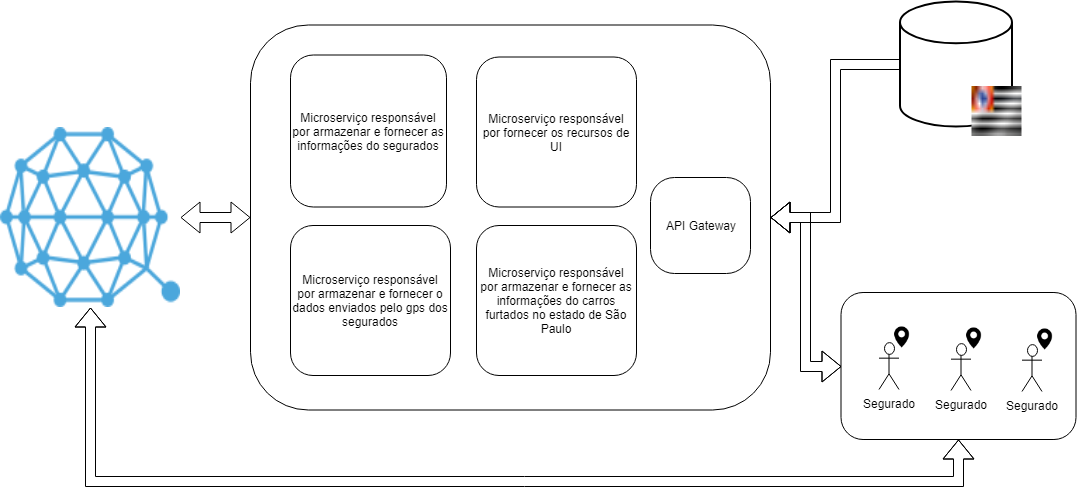
\includegraphics[width=0.8\textwidth]{Cap1/arquitetura_1}
\caption{Arquitetura 1: Todos os dados estão armazenados no blockchain.}
\label{arquitetura_1}
\end{figure}

\begin{figure}[ht]
\centering
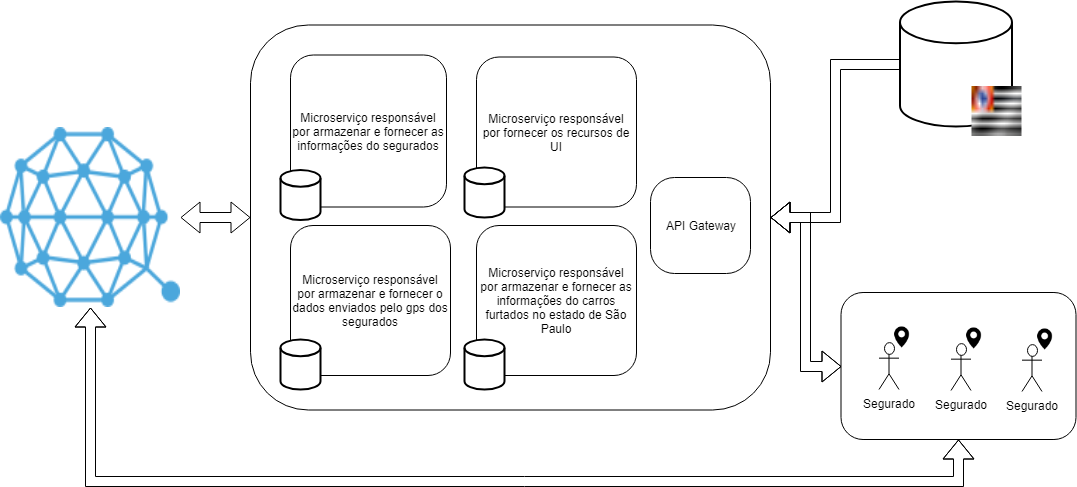
\includegraphics[width=0.8\textwidth]{Cap1/arquitetura_2}
\caption{Arquitetura 2: Parte dos dados está no blockchain e outra parte está em um banco de dados tradicional administrado pelo seguro.}
\label{arquitetura_2}
\end{figure}

\subsection{Partes envolvidas no seguro}

\begin{itemize}
\item Segurado: Responsável por
	\begin{itemize}
	\item Se cadastrar no seguro
    \item Enviar mensalmente a quantia acordada em Ethereum
    \item Instalar um dispositivo que envie em tempo real a localização de seu carro
    \item Iniciar o processo de reembolso em caso de roubo ou furto
	\end{itemize}
\item Seguro: Responsável por
	\begin{itemize}
	\item Disponibilizar um Website no qual as pessoas possam aderir ao seguro e acompanhar seus dados pessoais e os dados do seguro
    \item Criar e manter os contratos inteligentes na rede Ethereum
    \item Disponibilizar uma API para receber os dados de localização dos carros dos segurados
    \item Obter e cadastrar no sistema do seguro os carros furtados no Estado de São Paulo
	\end{itemize}
\item Governo do estado de São Paulo: Responsável por
	\begin{itemize}
	\item Disponibilizar um banco de dados com os dados de furtos e roubos de carros no Estado de São Paulo
	\end{itemize}
\end{itemize}

\subsection{O Contrato Inteligente}

O seguro será responsável por elaborar o código de dois contratos:

\begin{enumerate}
\item AutoInsuranceFactory: Responsável por
	\begin{itemize}
	\item Criar os contratos do seguro (AutoInsurance)
    \item Armazenar todos os contratos já criados e quem os criou
	\end{itemize}
\item AutoInsurance: Responsável por
	\begin{itemize}
	\item Armazenar o dinheiro enviado pelos segurados, em Ethereum
    \item Reembolsar o segurado em caso de roubo ou furto. O reembolso só será efetuado caso um boletim de ocorrência seja efetuado e disponibilizado no banco de dados do Governo do Estado de São Paulo. Um outro critério para a liberação do reembolso é o de que o local e hora do roubo ou furto registrado no B.O. coincida com os dados enviados pelo dispositivo instalado no carro do segurado.
	\end{itemize}
\end{enumerate}

\section{BIP32 \& BIP39}

Para garantir a privacidade dos usuários, os dados enviados pelo dispositivo GPS serão criptografados, de modo que cada amostra do sinal GPS será criptografado e descriptografado por uma mesma chave privada. Desse modo, o usuário terá o controle de privacidade de cada amostra, podendo fornecer a chave privada de amostras específicas do dispositivo GPS.

Para gerar múltiplas chaves privadas para cada amostra de sinal GPS é utilizado o BIP32.

\subsection{BIP32}

BIP32 \cite{github_bip32}, ``Bitcoin Improvement Proposal number 32'', é, de acordo com \cite{deployability_bitcoin_bip32}, uma técnica utilizada para geração de uma árvore de endereços bitcoin (chave pública e chave privada) a partir de uma chave semente, conhecida como ``Master Seed''. A partir da ``Master Seed'', um nó mestre é gerado e a partir do nó mestre, outros nós podem ser gerados. Na figura \ref{hd_tree}, pode-se ver o exemplo de uma árvore gerada pelo BIP32.

\begin{figure}[ht]
\centering
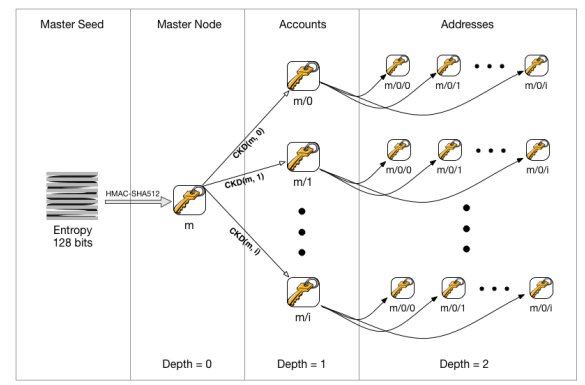
\includegraphics[width=0.9\textwidth]{Cap1/hd_tree}
\caption{BIP32: Árvore de endereços bitcoin.}
\label{hd_tree}
\end{figure}

\subsubsection{Chave extendida}

Para evitar que as chaves filhas dependam somente das chaves mãe, é utilizado o conceito de chaves extendidas. Uma chave extendida nada mais é do que uma chave pública ou privada acompanhada de 256 bits de entropia, esses 256 bits de entropia é conhecido como ``chain code''. Neste caso, uma chave privada extendida é obtida a partir do par ordenado (k, c), sendo k a chave privada e c o ``chain code''.

\subsubsection{Geração do nó mestre}

O nó mestre é obtido indiretamente a partir de S, também conhecido como ``master seed'':

\begin{enumerate}
\item Gerar uma sequência de bytes S (entre 128 e 512 bits);
\item Calcular I = HMAC-SHA512(Key = "Bitcoin seed", Data = S);
\item Separar I em duas arrays de 32 bytes, I = I\textsubscript{l} || I\textsubscript{r};
\item I\textsubscript{l} representará a chave privada mestre e I\textsubscript{r} representará o ``chain code''  mestre.
\end{enumerate}

\subsubsection{Geração de uma chave privada filha}

As chaves privadas filhas são geradas a partir da chave privada mãe extendida segundo a função: 
\[CKDpriv((k_{par}, c_{par}), i) \rightarrow (k_{i}, c_{i})\]

CKDpriv é obtido a paritr do seguintes passos:

\begin{enumerate}
\item Checar se i (índice do filho) é maior que 2\textsuperscript{31}:
  \begin{itemize}
  \item Se sim (``hardened child''), I = HMAC-SHA512(Key = c\textsubscript{par}, Data = 0x00 || ser\textsubscript{256}(k\textsubscript{par}) || ser\textsubscript{32}(i))
  \item Caso contrário (``normal child''), I = HMAC-SHA512(Key = c\textsubscript{par}, Data = ser\textsubscript{256}(k\textsubscript{par}) || ser\textsubscript{32}(i)) 
  \end{itemize}
\item Separar I em duas arrays de 32 bytes, I = I\textsubscript{l} || I\textsubscript{r};
\item k\textsubscript{i} = parse\textsubscript{256}(I\textsubscript{l}) + k\textsubscript{par} (mod n), onde n é ordem da curva secp256k1 \cite{secp256k1};
\end{enumerate}

\subsection{BIP39}

BIP39 \cite{github_bip39}, ``Bitcoin Improvement Proposal number 39'', é, de acordo com \cite{fornaro_thesis}, uma técnica utilizada para obter a ``Master seed'' a partir de uma frase mnemônica. Uma frase mnemônica nada mais é do que uma lista ordenada de palavras tiradas de determinado dicionário. Os passos para se obter o mnemônico  partir de uma entrada aleatória podem ser vistos na figura \ref{bip39_to_mnemonic} e os passos para se obter o ``Seed'' a partir do mnêmonico podem ser observados na figura \ref{bip39_to_seed}.

\begin{figure}[ht]
\centering
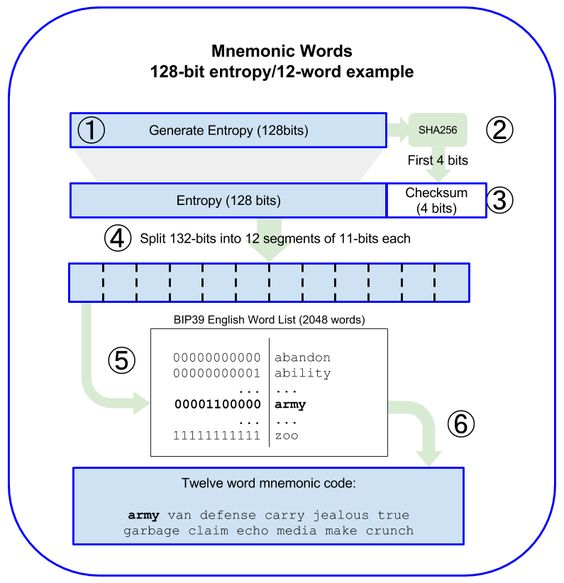
\includegraphics[width=0.8\textwidth]{Cap1/bip39_to_mnemonic}
\caption{Geração do mnemônico.}
\label{bip39_to_mnemonic}
\end{figure}

\begin{figure}[ht]
\centering
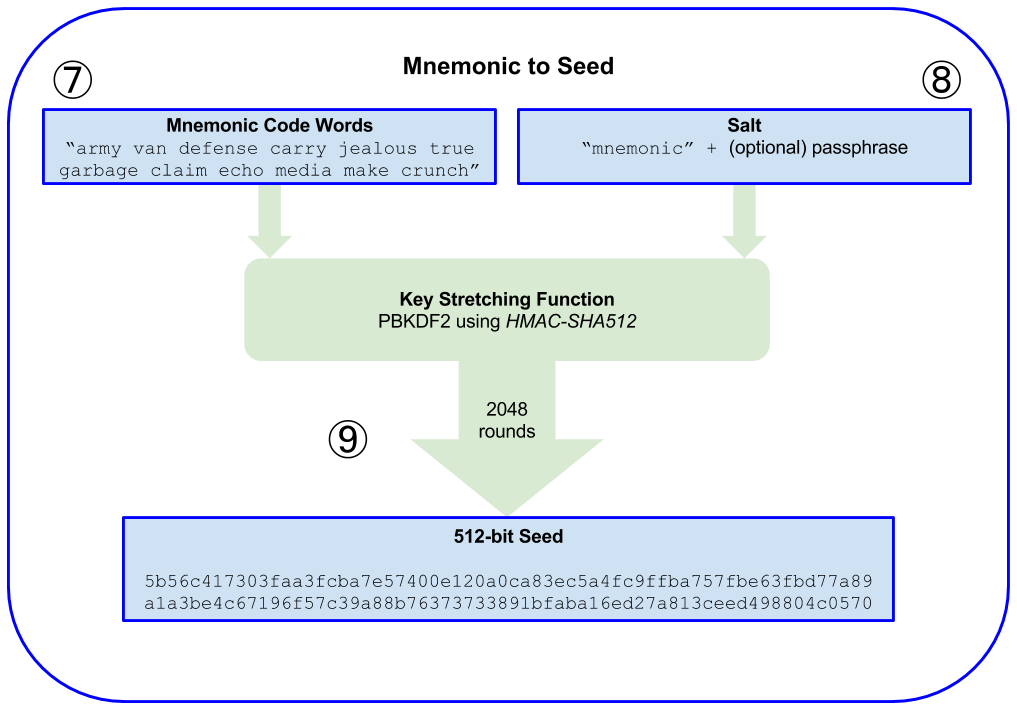
\includegraphics[width=0.8\textwidth]{Cap1/bip39_to_seed}
\caption{Obtenção do ``seed'' a partir do mnemônico.}
\label{bip39_to_seed}
\end{figure}

%vê o problema de controle tolerante a falhas através de uma perspectiva integrada, foi proposta por
%{marcel4}. Os autores apresentam um ambiente híbrido consistindo de três unidades básicas que garantem a compleição de tarefas na presença de qualquer número de juntas falhas (Figura \ref{cupim}). A primeira unidade é um esquema de detecção
%e isolação de falhas que continuamente monitora o manipulador para detectar e identificar possíveis falhas nas juntas. A segunda unidade é responsável pela reconfiguração do controle. A terceira unidade é composta de algorítmos de
%controle apropriados para cada tipo de configuração do robô, baseado na informação da unidade de reconfiguração \cite{COFFEE2000}.

%Segundo, o critério de otimização utilizado será o acoplamento entre as juntas do
%manipulador e neste caso, temos um sistema redundante quando ocorre falha de uma das juntas do manipulador de três juntas, e seu posicionamento é controlado pelas duas restantes. Nossa solução para o problema é baseada na formulação
%inversa ({nakamura}). A

%\begin{figure}[ht!]
%\centering
%\includegraphics[width=1\textwidth]{Cap1/cupimconcreto}
%\caption{Exemplo real de cupim frente ao seu dilema.}
%\label{FDII}
%\end{figure}